\chapter{Mehrdimensionale Integration}
Sei $f:D\rightarrow\R, D\subseteq \R^n$ eine stetige Funktion. Was ist $\int_D f=\int_D f(x)dx$?

\paragraph{Einfachster Fall}
$D$ ist ein Quader, d.h. es gibt $a_1,b_1,a_2,b_2,\ldots,a_n,b_n$ mit $a_i\leq b_i$. Dann ist
\begin{equation*}
	Q\coloneqq [a_1,b_1]\times \ldots\times [a_n,b_n]
\end{equation*}
ein Quader und man definiert für eine stetige Funktion $f:Q\rightarrow\R$
\begin{equation*}
	\int_Q f\coloneqq \int\limits_{a_n}^{b_n}\cdots\int\limits_{a_2}^{b_2}\int\limits_{a_1}^{b_1} f(x_1,\ldots,x_n)\intd x_1\intd x_2\ldots \intd x_n
\end{equation*}
(ohne Beweis der Wohldefiniertheit)

\paragraph{Beispiel:}
\begin{align*}
	&\quad\int\limits_0^2\int\limits_0^1 x*y\intd x \intd y\\
	&=\int\limits_0^2 \frac 12 x^2\Big|_0^1\intd y\\
	&=\frac 12 \int\limits_0^2 y\intd y\\
	&=\frac 12 \left(\frac12 y^2\right)\Bigg|_0^2\\
	&=1
\end{align*}

\paragraph{Bemerkung:}
Es kommt nicht auf die Reihenfolge der Variablen an
\begin{equation*}
	\int\limits_{a_2}^{b_2}\int\limits_{a_1}^{b_1} f(x_1,x_2)\intd x_1\intd x_2
	=\int\limits_{a_1}^{b_1}\int\limits_{a_2}^{b_2} f(x_1,x_2)\intd x_2\intd x_1
\end{equation*}

\section{Allgemeine Integrationsbereiche}
Oft werden sogenannte Normalbereiche, auch zylindrische Mengen benutzt:
\begin{itemize}
	\item Ein 1-dimensionaler Normalbereich ist ein Intervall $[a_1,b_1]$
	\item Seien $\phi_1,\psi_1:[a_1,b_1]\rightarrow \R$ stetig mit $\phi_1\leq \psi_1$. Ein zweidimensionaler Normalbereich $B$ ist gegeben durch
	\begin{equation*}
		B=\set{(x_1,x_2)\in\R}{x_1\in[a_1,b_1],\phi_1(x_1)\leq x_2\leq \psi_1(x_1)}
	\end{equation*}

	\begin{center}
		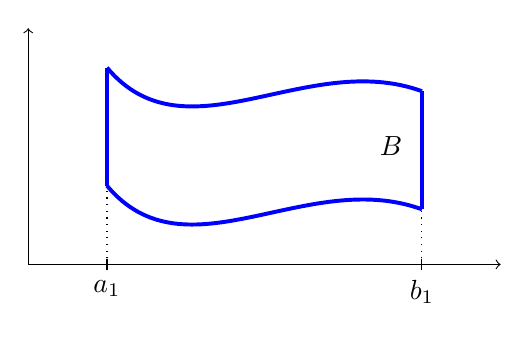
\begin{tikzpicture}
			\draw[black, ->] (0,0) to (6,0);
			\draw[black, ->] (0,0) to (0,3);

			\draw[blue, line width=0.5mm] (1,2.5) to[out=-50,in=160] (5,2.2);
			\draw[blue, line width=0.5mm] (1,1) to[out=-50,in=160] (5,0.7);

			\draw (5,1.5) node [draw=none, blue, label={left:$B$}] {};

			\draw (1,0) node (a) [draw, rectangle,minimum size=0pt,inner sep = 0pt, minimum height=4pt, label={below:$a_1$}] {};
			\draw (5,0) node (b) [draw, rectangle,minimum size=0pt,inner sep = 0pt, minimum height=4pt, label={below:$b_1$}] {};
			\draw[dotted]
			(a) -- (1,2.5)
			(b) -- (5,2.2);

			\draw[blue, line width=0.5mm] (1,2.5) -- (1,1) (5,2.2) -- (5,0.7);
		\end{tikzpicture}
	\end{center}


	\item Sei $B^k$ ein $(n-1)$-dimensionaler Normalbereich. $\phi_{n-1},\psi_{n-1}:B^k\rightarrow \R, \phi_{n-1}\leq\psi_{n-1}$. Dann ist ein $n$-dimensionaler Normalbereich gegeben durch
	\begin{equation*}
		B=\set{(x_1,\ldots,x_n)}{(x_1,\ldots,x_{n-1})\in B^k, \phi_{n-1}(x_1,\ldots,x_{n-1})\leq x_n\leq\psi_{n-1}(x_1,\ldots,x_{n-1})}
	\end{equation*}
\end{itemize}
Das Integral über eine stetige Funktion $f:B\rightarrow \R$ auf einem $n$-dimensionalen Normalbereich ist definiert durch
\begin{equation*}
	\int_Bf\coloneqq
	\int\limits_{a_1}^{b_1}
	\int\limits_{\phi_1(x_1)}^{\psi_1(x_1)}
	\cdots
	\int\limits_{\phi_{n-1}(x_1,\ldots,x_{n-1})}^{\psi_{n-1}(x_1,\ldots,x_{n-1})}f(x_1,\ldots,x_n)
	\intd x_n\ldots\intd x_2\intd x_1
\end{equation*}

\section{Der Transformationssatz}
Verallgemeinerung der Substitutionsregel aufs Mehrdimensionale


\begin{satz}{Transformationssatz}
	Sei $f:B\rightarrow \R$ stetig, $g:U\rightarrow B, U^n\subseteq \R^n$ eine Transformation, d.h. $g$ ist stetig differenzierbar und für die Funktionaldeterminante (Determinante der Jacobimatrix) gilt $\det Dg(x)=0$ für alle $x\in U$.
	$D=g^{-1}(B)$, dann gilt
	\begin{equation*}
		\int_B f(x)\intd x =\int_D f(g(u)) \det Dg(u)\intd u
	\end{equation*}
\end{satz}
Geometrische Interpretation von $\det Dg$, Volumenverzerrung.

\begin{center}
	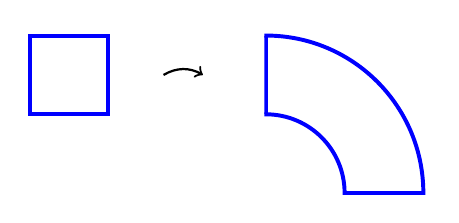
\begin{tikzpicture}
		\draw[blue, line width=0.5mm] (0,1) rectangle (1,2);

		\draw[black, thick, ->, bend left] (1.7,1.5) to (2.2,1.5);
		\begin{scope}
			\clip (2.98,-0.02) rectangle (5.1,2.1);


			\draw[blue, line width=0.5mm] (3,0) circle (1);
			\draw[blue, line width=0.5mm] (3,0) circle (2);
			\draw[blue, line width=0.5mm] (3,1) -- (3,2) (4,0) -- (5,0);
		\end{scope}
	\end{tikzpicture}
\end{center}

\paragraph{Beispiele:}
\begin{enumerate}
	\item Für die lineare Abbildung $A=\matrix{3&1\\0&1}$. Bildet Quadrat mit Fläche $1$ auf Parallelogramm mit Fläche $\det A=3$ ab.

	\begin{center}
		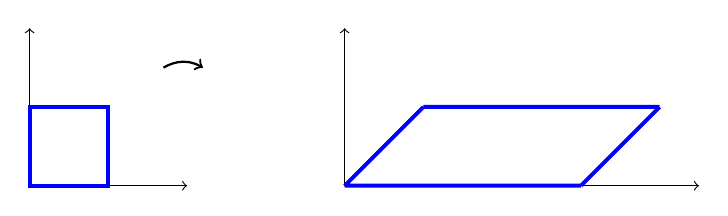
\begin{tikzpicture}
			\draw[black, ->] (0,0) to (2,0);
			\draw[black, ->] (0,0) to (0,2);

			\draw[blue, line width=0.5mm] (0,0) rectangle (1,1);

			\draw[black, thick, ->, bend left] (1.7,1.5) to (2.2,1.5);



			\draw[black, ->] (4,0) to (8.5,0);
			\draw[black, ->] (4,0) to (4,2);

			\draw[blue, line width=0.5mm]
			(4,0) -- (7,0)
			(5,1) -- (8,1)
			(4,0) -- (5,1)
			(7,0) -- (8,1);
		\end{tikzpicture}
	\end{center}
	\item Polarkoordinaten
	\begin{equation*}
		g(r,\varphi)=\vector{r\cos(\varphi)\\r\sin(\varphi)}, g:(0,\infty)\times (0,2\pi)\rightarrow \R^2
	\end{equation*}
	mit
	\begin{equation*}
		Dg(r,\phi)=\matrix{
		\cos(\varphi)&-r\sin(\varphi)\\
		\sin(\varphi)&r\cos(\varphi)}
	\end{equation*}

	$\det Dg(r,\phi)=r(\cos \varphi)^2+r(\sin\varphi)^2=r$
	Flächeninhalt des Kreises mit Radius $R$, $D=(0,R)\times(0,2\pi)$
	\begin{align*}
		\int_{K_R(0)}1\intd x=\int\limits_0^R\int\limits_0^{2\pi} 1*\det Dg()
	\end{align*}
\end{enumerate}
